\documentclass[12pt,a4paper]{report}
\usepackage[a4paper,margin=1in,headheight=15pt]{geometry}
\usepackage{fontspec}
\setmainfont{texgyretermes-regular.otf}[BoldFont=texgyretermes-bold.otf,ItalicFont=texgyretermes-italic.otf,BoldItalicFont=texgyretermes-bolditalic.otf]
\setsansfont{texgyreheros-regular.otf}[BoldFont=texgyreheros-bold.otf,ItalicFont=texgyreheros-italic.otf,BoldItalicFont=texgyreheros-bolditalic.otf]
\setmonofont{texgyrecursor-regular.otf}[BoldFont=texgyrecursor-bold.otf,ItalicFont=texgyrecursor-italic.otf,BoldItalicFont=texgyrecursor-bolditalic.otf,Scale=MatchLowercase]
\usepackage{graphicx}
\usepackage{booktabs,array,tabularx,longtable}
\usepackage{amsmath}
\usepackage{xcolor}
\usepackage{setspace}
\usepackage{fancyhdr}
\usepackage{caption}
\usepackage{enumitem}
\usepackage{titlesec}
\usepackage[hidelinks]{hyperref}
\graphicspath{{../assets/figs/}{../assets/screens/}}
\setstretch{1.25}
\captionsetup{font=small,labelfont=bf}
\setlist{itemsep=2pt,topsep=4pt}
\titleformat{\chapter}[display]{\normalfont\huge\bfseries}{\chaptertitlename\ \thechapter}{14pt}{\Huge}
\titlespacing*{\chapter}{0pt}{-20pt}{24pt}
\definecolor{accent}{HTML}{D95926}
\definecolor{navy}{HTML}{131A2B}
\pagestyle{fancy}
\fancyhf{}
\fancyhead[L]{\small ReviewIQ: Project Report}
\fancyhead[R]{\small Vidyalankar Institute of Technology}
\fancyfoot[C]{\thepage}
\renewcommand{\headrulewidth}{0.4pt}
\fancypagestyle{plain}{\fancyhf{}\fancyfoot[C]{\thepage}\renewcommand{\headrulewidth}{0pt}}
\newcommand{\fig}[3]{\begin{figure}[htbp]\centering\includegraphics[width=#2]{#1}\caption{#3}\end{figure}}

\begin{document}

% ------------------------------------------------------------------ TITLE
\begin{titlepage}
\thispagestyle{empty}
\centering
{\Large\bfseries\color{navy} VIDYALANKAR INSTITUTE OF TECHNOLOGY\par}
\vspace{2pt}
{\large Mumbai, India\par}
\vspace{1.2cm}
\rule{\textwidth}{1.2pt}\par
\vspace{0.6cm}
{\Huge\bfseries\color{accent} ReviewIQ\par}
\vspace{0.3cm}
{\LARGE\bfseries AI-Based Product Review Intelligence\\ and Consumer Insight System\par}
\vspace{0.4cm}
{\large Sentiment classification with NLP, deep learning and advanced machine learning,\\ aspect intelligence, review trust analysis and grounded question answering\par}
\vspace{0.6cm}
\rule{\textwidth}{1.2pt}\par
\vspace{1.2cm}
{\large\bfseries Project Report\par}
\vspace{0.8cm}
{\large Submitted by\par}
\vspace{0.4cm}
\begin{tabular}{lr}
\textbf{Nidhi Bhawari} & 23102A0006 \\[4pt]
\textbf{Aarti Sakpal} & 23102A0007 \\[4pt]
\textbf{Gayatri Patil} & 23102A0016 \\[4pt]
\textbf{Prachi Wakode} & 23102A0020 \\
\end{tabular}
\vspace{1.2cm}

{\large Under the guidance of\par}
\vspace{0.3cm}
{\Large\bfseries Prof. Sneha Annappanavar\par}
\vfill
{\large Vidyalankar Institute of Technology\par}
\end{titlepage}

% ------------------------------------------------------------------ CERTIFICATE
\chapter*{Certificate}
\addcontentsline{toc}{chapter}{Certificate}
\vspace{0.5cm}
This is to certify that the project report entitled \textbf{``ReviewIQ: AI-Based Product Review Intelligence and Consumer Insight System''} is a bonafide record of the work carried out by

\begin{center}
\begin{tabular}{ll}
Nidhi Bhawari & 23102A0006 \\
Aarti Sakpal & 23102A0007 \\
Gayatri Patil & 23102A0016 \\
Prachi Wakode & 23102A0020 \\
\end{tabular}
\end{center}

at \textbf{Vidyalankar Institute of Technology} under my guidance, and is submitted in partial fulfilment of the requirements of the project course.

\vspace{2.8cm}
\noindent
\begin{tabular}{@{}p{0.31\textwidth}p{0.31\textwidth}p{0.31\textwidth}@{}}
\rule{0.9\linewidth}{0.4pt} & \rule{0.9\linewidth}{0.4pt} & \rule{0.9\linewidth}{0.4pt} \\
\textbf{Prof. Sneha Annappanavar} & \textbf{Head of Department} & \textbf{Principal} \\
Project Guide & & \\
\end{tabular}

\vspace{2.2cm}
\noindent
\begin{tabular}{@{}p{0.45\textwidth}p{0.45\textwidth}@{}}
\rule{0.9\linewidth}{0.4pt} & \rule{0.9\linewidth}{0.4pt} \\
\textbf{Internal Examiner} & \textbf{External Examiner} \\
\end{tabular}
\clearpage

% ------------------------------------------------------------------ DECLARATION
\chapter*{Declaration}
\addcontentsline{toc}{chapter}{Declaration}
We declare that this written submission represents our ideas in our own words and that, where others' ideas or words have been included, we have adequately cited and referenced the original sources. We also declare that we have adhered to all principles of academic honesty and integrity and have not misrepresented, fabricated or falsified any idea, data, fact or source in our submission.

\vspace{1.5cm}
\noindent
\begin{tabular}{@{}lll@{}}
\textbf{Nidhi Bhawari} & 23102A0006 & \rule{4cm}{0.4pt} \\[18pt]
\textbf{Aarti Sakpal} & 23102A0007 & \rule{4cm}{0.4pt} \\[18pt]
\textbf{Gayatri Patil} & 23102A0016 & \rule{4cm}{0.4pt} \\[18pt]
\textbf{Prachi Wakode} & 23102A0020 & \rule{4cm}{0.4pt} \\
\end{tabular}
\clearpage

% ------------------------------------------------------------------ ACKNOWLEDGEMENT
\chapter*{Acknowledgement}
\addcontentsline{toc}{chapter}{Acknowledgement}
We would like to express our sincere gratitude to our project guide, \textbf{Prof. Sneha Annappanavar}, for her guidance, encouragement and constructive feedback throughout the course of this project. Her suggestions helped us shape the problem, choose the right evaluation methods and present the work clearly.

We thank \textbf{Vidyalankar Institute of Technology} for providing the facilities and environment needed to carry out this work. We are also grateful to the maintainers of the Amazon Reviews 2023 collection and to the open-source communities behind PyTorch, scikit-learn, XGBoost, Hugging Face Transformers, Sentence-Transformers and Streamlit, whose tools made this project possible.

Finally, we thank our families and friends for their support.

\clearpage

% ------------------------------------------------------------------ ABSTRACT
\chapter*{Abstract}
\addcontentsline{toc}{chapter}{Abstract}
Online product reviews are abundant but unstructured, and a single popular product can attract thousands of opinions that no person can read in full. This project, \textbf{ReviewIQ}, turns raw Amazon Electronics reviews into decisions for two audiences: buyers who ask ``should I buy this?'' and sellers who ask ``what should we improve?''.

The system combines three families of techniques on one shared, metadata-enriched corpus of 50,000 reviews covering 34,365 products. The \textbf{NLP} branch uses a VADER lexicon baseline, TF-IDF with logistic regression and a linear SVM, LDA topic modelling and aspect-based sentiment analysis. The \textbf{deep learning} branch trains a bidirectional LSTM with attention from scratch and fine-tunes DistilBERT. The \textbf{advanced machine learning} branch predicts review helpfulness with tuned XGBoost, clusters reviews with MiniBatchKMeans and flags potentially suspicious reviews with an unsupervised Isolation Forest. A semantic search and retrieval-augmented question-answering layer lets users ask product-specific questions and always shows the supporting reviews. Everything is delivered through a nine-page interactive Streamlit dashboard with a live sentiment classifier.

On a shared test set of 10,000 reviews, the BiLSTM reaches 88.8\% accuracy and the highest macro-F1 (0.718), significantly above a TF-IDF SVM, while DistilBERT reaches the highest accuracy (89.9\%) using only 6,000 training reviews. A three-seed ablation shows that class weighting, not attention, accounts for most of the LSTM's macro-F1 gain, and that an unweighted LSTM matches DistilBERT's accuracy. The LSTM is about 57 times faster than DistilBERT on a CPU with 26 times fewer parameters. Battery is the most criticised aspect (20.2\% negative mentions). A similarity-floor guardrail makes the question-answering component decline 95.6\% of plausible but unanswerable questions and 100\% of off-topic ones, while accepting 97.8\% of answerable questions. Limitations, including weak labels from star ratings and a non-random sample, are stated explicitly.

\medskip
\noindent\textbf{Keywords:} sentiment analysis, LSTM, attention, DistilBERT, aspect-based sentiment analysis, XGBoost, Isolation Forest, retrieval-augmented generation, product reviews.
\clearpage

\tableofcontents
\clearpage
\listoffigures
\clearpage
\listoftables
\clearpage

% ------------------------------------------------------------------ ABBREVIATIONS
\chapter*{List of Abbreviations}
\addcontentsline{toc}{chapter}{List of Abbreviations}
\begin{tabular}{@{}p{3.2cm}p{11cm}@{}}
\textbf{ABSA} & Aspect-Based Sentiment Analysis \\
\textbf{AML} & Advanced Machine Learning \\
\textbf{ASIN} & Amazon Standard Identification Number \\
\textbf{BiLSTM} & Bidirectional Long Short-Term Memory \\
\textbf{CI} & Confidence Interval \\
\textbf{DL} & Deep Learning \\
\textbf{LDA} & Latent Dirichlet Allocation \\
\textbf{LSTM} & Long Short-Term Memory \\
\textbf{NLP} & Natural Language Processing \\
\textbf{RAG} & Retrieval-Augmented Generation \\
\textbf{SVM} & Support Vector Machine \\
\textbf{TF-IDF} & Term Frequency, Inverse Document Frequency \\
\textbf{VADER} & Valence Aware Dictionary and sEntiment Reasoner \\
\textbf{XGBoost} & Extreme Gradient Boosting \\
\end{tabular}
\clearpage

% ================================================================== CH 1
\chapter{Introduction}
\section{Background and Motivation}
Customer reviews influence purchasing decisions and guide product development. On a large marketplace, however, a popular product can have thousands of free-text opinions, and the star average hides what customers actually say. A buyer wants to know what people like and dislike about \emph{this} product. A seller wants to know which problems recur across products and which reviews are worth reading. Reading everything is impossible, so automated review analysis is central to modern e-commerce.

The problems involved are usually studied separately: sentiment classification, aspect extraction, helpfulness prediction and opinion-spam detection often use different datasets and evaluation protocols. It is therefore hard to judge what each family of methods (lexicon and feature-based NLP, neural sequence models, ensemble and unsupervised learning) contributes to a practical system.

\section{Problem Statement}
To design, implement and evaluate an end-to-end system that classifies customer review sentiment into positive, neutral and negative classes, extracts aspect-level insight, assesses review quality and trust, and answers natural-language questions about a product using only its own reviews, serving both buyers and businesses through one interactive interface.

\section{Objectives}
\begin{enumerate}
\item Prepare a clean, labelled review corpus enriched with product names, brands and images.
\item Classify review sentiment with models from three families (NLP, deep learning and advanced ML) and compare them fairly on one test set.
\item Build an LSTM-based sentiment classifier, report its performance metrics and visualise the language of each sentiment with word clouds.
\item Derive aspect-level sentiment, topics and clusters to show what customers talk about and complain about.
\item Predict review helpfulness and flag potentially suspicious reviews.
\item Provide semantic search and a grounded question-answering interface that shows its evidence and declines unsupported questions.
\item Deliver all results through a dashboard for buyers, businesses and model inspection.
\end{enumerate}

\section{Scope}
The project covers one product category (Amazon Electronics), English-language reviews, and a 50,000-review working sample. Sentiment labels are derived from star ratings. Suspicious-review detection is unsupervised and makes no claim of identifying fake reviews with a measured accuracy.

\section{Contributions}
\begin{itemize}
\item A three-pillar framework integrating NLP, deep learning and advanced machine learning over a shared corpus.
\item A like-for-like comparison of five sentiment models with bootstrap confidence intervals and paired significance tests.
\item A three-seed ablation separating the effect of attention pooling from that of class weighting, and a measured cost comparison.
\item Product-level intelligence: aspect complaint ranking, helpfulness prediction and a corrected unsupervised suspicious-review score.
\item Grounded question answering with a similarity floor whose effect is measured.
\item A candid account of limitations and of the engineering problems found and fixed during development.
\end{itemize}

\section{Organisation of the Report}
Chapter 2 surveys related work. Chapter 3 presents the analysis and design. Chapter 4 describes the dataset. Chapter 5 explains the implementation. Chapter 6 reports testing and results. Chapter 7 concludes and lists future work. Appendices show dashboard screenshots and how to run the project.

% ================================================================== CH 2
\chapter{Literature Survey}
\section{Sentiment Classification}
Early work framed review sentiment as supervised classification with bag-of-words features \cite{pang2002thumbs}, where linear support vector machines remain a strong baseline \cite{joachims1998text}. Lexicon-and-rule systems such as VADER \cite{hutto2014vader} need no training data and are a common zero-shot baseline. Recurrent networks, notably the LSTM \cite{hochreiter1997lstm}, model word order and negation, and attention mechanisms \cite{bahdanau2015attention} let a classifier weight the most informative tokens; attention-based LSTMs were applied to aspect-level sentiment by Wang et al.\ \cite{wang2016attention}. Pre-trained transformers \cite{devlin2019bert}, including the distilled DistilBERT \cite{sanh2019distilbert}, now dominate benchmarks.

\section{Aspects, Topics and Review Quality}
Feature-level opinion mining \cite{hu2004mining} extracts product aspects and the sentiment expressed towards them, and topic models such as LDA \cite{blei2003lda} discover themes without labels. Helpfulness has been predicted from structural, lexical and metadata features \cite{kim2006automatically}, which suits gradient-boosted trees \cite{chen2016xgboost}. Opinion spam is hard to study because labelled ground truth is scarce \cite{jindal2008opinion,ott2011finding}; unsupervised outlier detection such as Isolation Forest \cite{liu2008isolation} is a pragmatic option when no labels exist.

\section{Retrieval and Grounded Generation}
Sentence encoders \cite{reimers2019sbert,wang2020minilm} retrieve by meaning rather than keyword overlap, and retrieval-augmented generation \cite{lewis2020rag} conditions a generator on retrieved passages so that answers can be traced to evidence. Instruction-tuned encoder-decoder models \cite{raffel2020t5,chung2022flan} are small enough to run locally. A known weakness is that generators may answer confidently even when retrieval is weak.

\section{Summary of Gaps Addressed}
\begin{table}[htbp]
\centering
\caption{Gaps in typical review-analysis work and how this project addresses them.}
\small
\begin{tabularx}{\textwidth}{@{}>{\raggedright\arraybackslash}p{4.3cm}X@{}}
\toprule
Typical gap & How ReviewIQ addresses it \\
\midrule
Tasks studied in isolation & One corpus feeds sentiment, aspects, helpfulness, trust and question answering \\
Single models reported as point estimates & Five models on one test split with bootstrap intervals and paired tests \\
Product identified by cryptic ID & Product names, brands and images joined via the parent ASIN \\
Opinion-spam claims without ground truth & Unsupervised score with explicit wording and no accuracy claim \\
Generated answers without evidence & Retrieved reviews always shown; similarity floor declines unsupported questions \\
\bottomrule
\end{tabularx}
\end{table}

% ================================================================== CH 3
\chapter{System Analysis and Design}
\section{Requirements}
\subsection{Functional requirements}
\begin{itemize}
\item Load, clean and label a review corpus and join product metadata.
\item Classify the sentiment of any review text with several models and report metrics.
\item Show, per product, a summary, aspect sentiment with supporting sentences, filterable reviews and review-trust analysis.
\item Compare two products using computed statistics only.
\item Answer product-specific questions from that product's reviews and show the evidence.
\item Provide corpus-wide business views: complaint ranking, topics, clusters, helpfulness and suspicious reviews.
\item Provide a model-inspection area with metrics, training curves, word clouds and a live classifier.
\end{itemize}
\subsection{Non-functional requirements}
Responsiveness (pages must render in seconds, with heavy computation cached), explainability (every insight links to evidence), honesty (limitations and uncertainty stated), no login or personal data, and reproducibility (every reported number regenerated by a script).

\section{System Architecture}
Figure~\ref{fig:framework} shows the architecture. Cleaned and labelled reviews feed three parallel branches whose outputs are fused into product-level intelligence and a semantic search and retrieval-augmented question-answering layer, all exposed through one dashboard.
\begin{figure}[htbp]\centering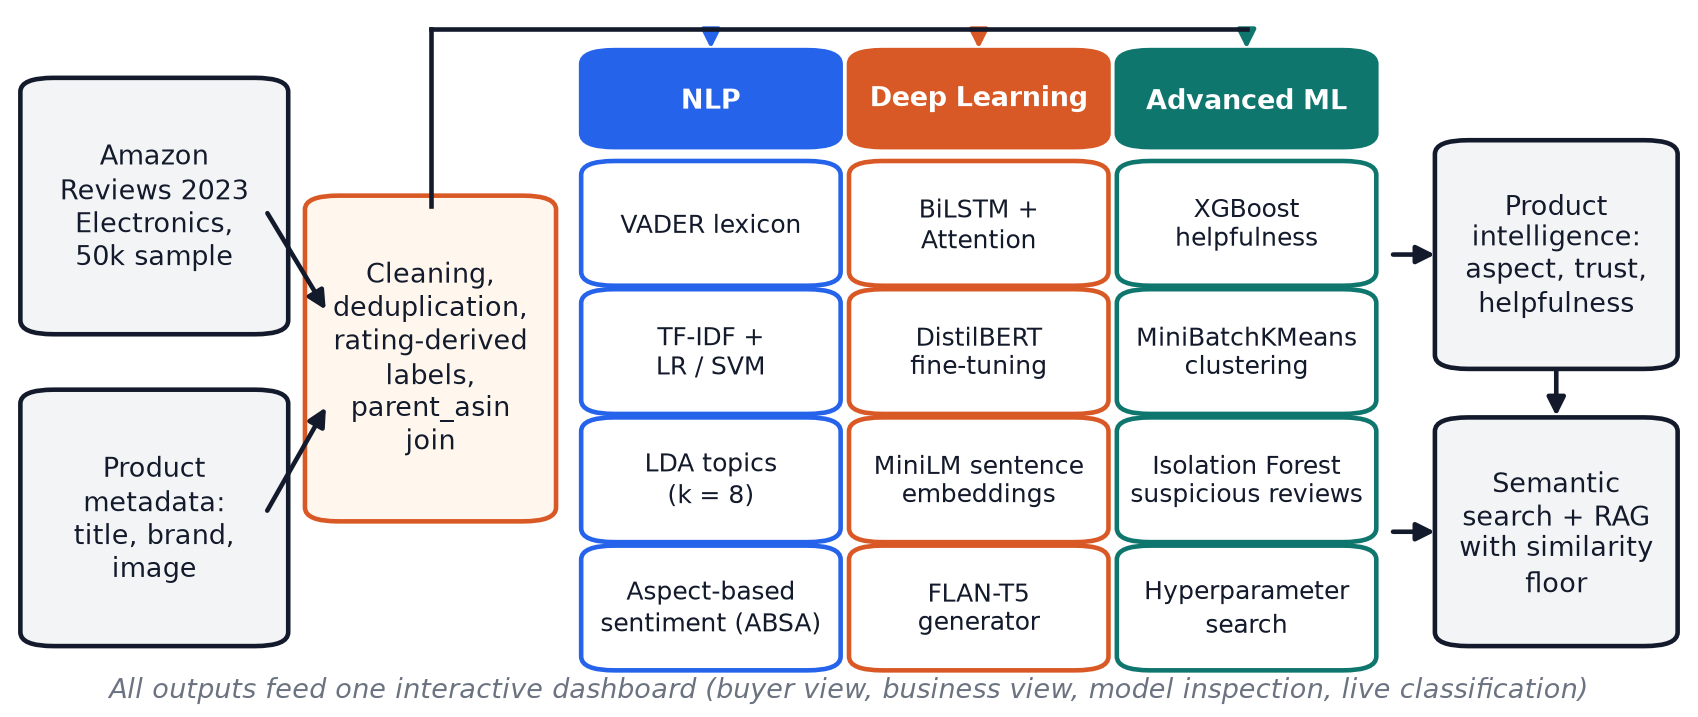
\includegraphics[width=\textwidth]{fig_framework.png}\caption{Overall architecture of ReviewIQ.}\label{fig:framework}\end{figure}

\section{Data Flow}
\begin{enumerate}
\item Raw review records are read, cleaned, de-duplicated and labelled (positive, neutral, negative from star ratings), producing the processed review table.
\item Product metadata (title, brand, image) is fetched and joined on the parent ASIN, producing the products table. Reviews are never duplicated per product attribute.
\item Each branch reads the processed table and writes its own artefacts: models, prediction tables, metrics reports and figures.
\item All reviews are encoded once into sentence embeddings that are reused by semantic search, the question-answering layer and the suspicious-review feature that measures near-duplicate text.
\item The dashboard loads the tables and artefacts, joins them by product, and renders each page. Heavy computations are cached.
\end{enumerate}

\section{Module Description}
\begin{table}[htbp]
\centering
\caption{Modules of the system.}
\small
\begin{tabularx}{\textwidth}{@{}>{\raggedright\arraybackslash}p{3.6cm}X@{}}
\toprule
Module & Responsibility \\
\midrule
Data preparation & Cleaning, de-duplication, sampling, rating-derived labels, metadata join \\
NLP & VADER, TF-IDF with logistic regression and SVM, LDA topics, aspect-based sentiment \\
Deep learning & BiLSTM with attention, fine-tuned DistilBERT, word clouds, live classifier \\
Advanced ML & XGBoost helpfulness, MiniBatchKMeans clustering, Isolation Forest suspicious reviews \\
Semantic search and RAG & Sentence embeddings, product-scoped retrieval, FLAN-T5 answers, similarity floor \\
Dashboard & Nine Streamlit pages for buyers, businesses and model inspection \\
Evaluation & Shared-split metrics, bootstrap intervals, ablation, cost, retrieval and guardrail experiments \\
\bottomrule
\end{tabularx}
\end{table}

\section{Technology Stack}
\begin{table}[htbp]
\centering
\caption{Technologies used.}
\small
\begin{tabularx}{\textwidth}{@{}>{\raggedright\arraybackslash}p{4.2cm}X@{}}
\toprule
Purpose & Tools \\
\midrule
Language and data & Python 3.12, pandas, NumPy \\
Classical ML & scikit-learn 1.9, XGBoost 3.4 \\
Deep learning & PyTorch 2.13 (CUDA), Hugging Face Transformers 5.16 \\
Sentiment baseline & vaderSentiment \\
Embeddings and retrieval & Sentence-Transformers (all-MiniLM-L6-v2) \\
Generation & FLAN-T5-base \\
Visualisation & Matplotlib, wordcloud \\
User interface & Streamlit 1.62 with custom CSS \\
Testing and capture & Streamlit AppTest, Playwright \\
Documents & LaTeX (Tectonic), python-pptx \\
\bottomrule
\end{tabularx}
\end{table}

\section{Environment}
Training and evaluation were run on a laptop with an NVIDIA GeForce RTX 4050 Laptop GPU (6 GB) and an 8-thread CPU under Linux (WSL2). DistilBERT was fine-tuned on CPU.

% ================================================================== CH 4
\chapter{Dataset and Preprocessing}
\section{Dataset}
The Electronics category of the Amazon Reviews 2023 collection (McAuley Lab) \cite{hou2024bridging} was used. A working sample of 50,000 reviews was prepared. Table~\ref{tab:data} summarises it.
\begin{table}[htbp]
\centering
\caption{Statistics of the 50,000-review working sample.}\label{tab:data}
\begin{tabular}{@{}ll@{}}
\toprule
Property & Value \\
\midrule
Reviews / products / reviewers & 50,000 / 34,365 / 8,883 \\
Review dates & 2000 to March 2023 \\
Mean / median length (words) & 71.7 / 39 \\
Mean star rating & 4.25 \\
Verified purchases & 80.2\% \\
Reviews with at least one helpful vote & 26.2\% \\
Positive / neutral / negative & 40,205 / 3,506 / 6,289 \\
\quad share of corpus & 80.4\% / 7.0\% / 12.6\% \\
Products matched to metadata & 34,364 / 34,365 \\
\bottomrule
\end{tabular}
\end{table}

\section{Cleaning Steps}
Records without a rating, or with fewer than three words after cleaning, were dropped. HTML entities, tags and URLs were removed. Duplicate (reviewer, product, text) triples were removed. The review title and body were concatenated into one text field. The sample was stratified by sentiment class and shuffled with a fixed seed.

\section{Labels}
Sentiment labels are weakly supervised from star ratings: ratings of 4 and 5 are positive, 3 is neutral, and 1 and 2 are negative. This is standard practice at scale but introduces label noise: a three-star review can be warm, and a five-star review can contain a complaint. Because the classes are strongly imbalanced, macro-averaged F1 is used as the primary metric.

\section{Product Metadata Integration}
Reviews carry only a product identifier. The category's metadata file (about 5.2 GB) was streamed and filtered to the parent ASINs present in the sample. Title, brand, image and category were joined on the parent ASIN, matching 34,364 of 34,365 products, and stored in a separate products table. Grouping by parent ASIN (the product listing) rather than the variant-level ASIN means colour and size variants roll up into one product.

\section{Sampling Caveat}
The working sample was taken from the beginning of the category file rather than drawn at random. That file is grouped by reviewer (the 65,552 raw records form 9,686 contiguous blocks, one per reviewer), so the sample over-represents prolific reviewers: 392 accounts with at least 20 reviews contribute about 40\% of it. This is discussed again where it affects the suspicious-review feature.

% ================================================================== CH 5
\chapter{Implementation}
\section{NLP Branch}
\subsection{VADER baseline}
VADER produces a compound score between $-1$ and $1$. Scores of at least 0.05 are labelled positive, at most $-0.05$ negative, and the rest neutral. It needs no training and serves as the zero-shot baseline.
\subsection{TF-IDF with logistic regression and linear SVM}
Reviews are vectorised with TF-IDF using unigrams and bigrams, 30,000 features, minimum document frequency 2 and sublinear term frequency. A multinomial logistic regression and a linear SVM are trained with balanced class weights on the 40,000-review training split.
\subsection{LDA topic modelling}
LDA with eight topics is fit with online variational inference on a count matrix of 3,000 unigram and bigram features (stop words removed), using an 8,000-document subsample for fitting and applying the model to all reviews. Table~\ref{tab:lda} lists the topics.
\begin{table}[htbp]
\centering
\caption{LDA topics and their leading words.}\label{tab:lda}
\small
\begin{tabularx}{\textwidth}{@{}c>{\raggedright\arraybackslash}p{3.7cm}X@{}}
\toprule
\# & Interpretation & Top words \\
\midrule
0 & Audio and speakers & sound, speaker, music, speakers, audio, bluetooth, quality, volume \\
1 & Storage cards, Apple accessories & card, ipad, cord, apple, sd, charging, sd card, phone, waste \\
2 & General praise, computers, drives & great, works, works great, drive, price, screen, computer \\
3 & USB and power accessories & usb, power, laptop, mouse, nice, good, work \\
4 & Cameras, TVs, mounts & camera, tv, light, video, mount, easy \\
5 & Cases and tablets & case, fit, perfect, love, tablet, keyboard \\
6 & Headphones and phones & great, sound, phone, quality, headphones, work, easy \\
7 & Cables and networking & cable, cables, router, wifi, hdmi, devices, signal \\
\bottomrule
\end{tabularx}
\end{table}
\subsection{Aspect-based sentiment analysis}
Ten aspects (battery, camera, display, sound, performance, build quality, price and value, connectivity, size and comfort, customer service) are defined by keyword lexicons. Each review is split into sentences; sentences containing an aspect keyword are scored with VADER, and the aspect receives a positive, neutral or negative polarity. The matched sentences are kept as human-readable evidence, so every aspect judgement in the interface can be inspected.

\section{Deep Learning Branch}
\subsection{BiLSTM with attention}
Tokens (lower-cased alphanumerics plus ``!'' and ``?'') are mapped to a vocabulary built on the training split only (14,937 words, minimum frequency 3), and sequences are truncated to 200 tokens (Figure~\ref{fig:lstmarch}). A learned 128-dimensional embedding feeds a two-layer bidirectional LSTM with 128 units per direction. With hidden states $\mathbf{h}_t$, attention pooling computes
\begin{equation}
\alpha_t=\frac{\exp(\mathbf{w}^{\top}\mathbf{h}_t)}{\sum_s \exp(\mathbf{w}^{\top}\mathbf{h}_s)},\qquad \mathbf{c}=\sum_t \alpha_t \mathbf{h}_t ,
\end{equation}
with padding masked, and $\mathbf{c}$ passes through dropout and a linear layer to a three-way softmax. Because the classes are imbalanced, the loss uses class weights $w_c=\sqrt{N/(3n_c)}$, and the best epoch is chosen by validation macro-F1 rather than loss.
\begin{figure}[htbp]\centering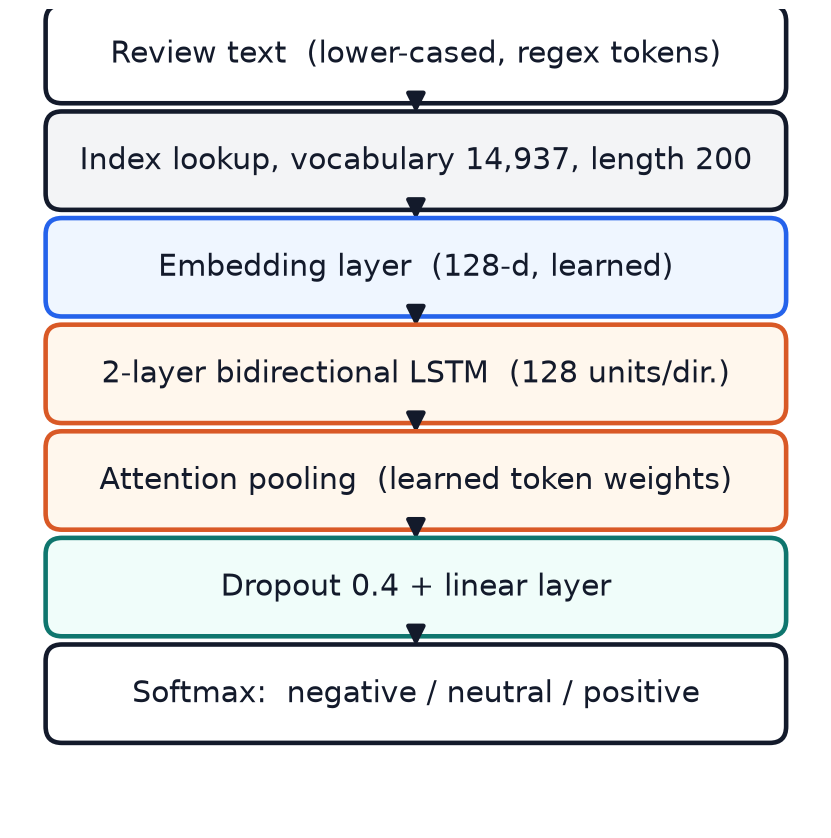
\includegraphics[width=0.55\textwidth]{fig_lstm_arch.png}\caption{Architecture of the BiLSTM with attention pooling.}\label{fig:lstmarch}\end{figure}
\begin{table}[htbp]
\centering
\caption{BiLSTM configuration.}
\small
\begin{tabular}{@{}ll@{}}
\toprule
Setting & Value \\
\midrule
Vocabulary / maximum length & 14,937 / 200 tokens \\
Embedding / hidden size / layers & 128 / 128 per direction / 2 \\
Trainable parameters & 2,572,420 \\
Optimiser & Adam, learning rate $2\times10^{-3}$, weight decay $10^{-5}$ \\
Batch size / gradient clipping & 128 / 1.0 \\
Dropout & 0.4 \\
Epochs / early stopping & at most 12 / patience 3 on validation macro-F1 \\
Training / validation / test reviews & 36,000 / 4,000 / 10,000 \\
Training time & about 7 minutes on a laptop GPU \\
\bottomrule
\end{tabular}
\end{table}
\subsection{Fine-tuned DistilBERT}
The pre-trained distilled transformer is fine-tuned with a three-way classification head (maximum length 128, AdamW optimiser, learning rate $2\times10^{-5}$, 2 epochs, batch size 8) on a stratified 6,000-review subsample, because the run was performed on a CPU (about 60 minutes).
\subsection{Word clouds and live classifier}
Word clouds are drawn per sentiment class, weighting each word by its within-class frequency multiplied by its over-representation relative to the whole corpus, so that distinctive rather than merely frequent vocabulary is shown. The dashboard's live classifier runs the LSTM, DistilBERT and the SVM side by side on any text and highlights the words the LSTM attended to.

\section{Advanced Machine Learning Branch}
\subsection{XGBoost helpfulness prediction}
The target is whether a review received at least one helpful vote. Ten engineered features are used (Table~\ref{tab:xgbfeat}). The model is tuned with 15 randomised-search candidates under 3-fold cross-validation optimising F1, with the positive-class weight set for the imbalance.
\begin{table}[htbp]
\centering
\caption{Features of the helpfulness model.}\label{tab:xgbfeat}
\small
\begin{tabularx}{\textwidth}{@{}>{\raggedright\arraybackslash}p{4.2cm}X@{}}
\toprule
Feature & Meaning \\
\midrule
rating & Star rating \\
review\_length\_words, title\_length\_words & Length of the review body and title \\
verified\_purchase & Verified-purchase flag \\
exclamation\_count, question\_count & Count of ``!'' and ``?'' \\
capital\_ratio & Share of capital letters \\
vader\_compound & VADER sentiment of the text \\
review\_age\_days & Age relative to the newest review \\
num\_aspects\_mentioned & Distinct aspects found by the ABSA module \\
\bottomrule
\end{tabularx}
\end{table}
\subsection{MiniBatchKMeans clustering}
Six clusters are computed on a separate TF-IDF representation (5,000 features, stop words removed) so that function words do not dominate.
\subsection{Isolation Forest for suspicious reviews}
With no labelled fake or genuine reviews, suspicious-review detection is framed as unsupervised anomaly detection. Features are a binary indicator for very short reviews, capital-letter ratio, exclamation count, verified-purchase flag, the logarithm of the number of reviews the same account has in the sample, and the maximum cosine similarity to another review of the same product (computed per product on sentence embeddings). After standardisation, an Isolation Forest with contamination 0.10 produces an anomaly score rescaled to $[0,1]$. A rule-based reason string accompanies each flag. The interface calls flagged reviews only ``potentially suspicious based on automated pattern analysis''.

\section{Semantic Search and Question Answering}
All reviews are encoded once with a MiniLM sentence encoder into 384-dimensional unit vectors, so cosine similarity is a dot product. For a question about a product, retrieval is restricted to that product's reviews and the top five by cosine similarity are returned. FLAN-T5-base is prompted with the question and the retrieved text (each review truncated to 300 characters) and asked to answer in one or two sentences using only that text. Small generators do not reliably follow ``say you do not know'' instructions, so a hard \emph{similarity floor} is applied: if the best similarity is below 0.30, the system answers that the reviews do not provide enough information and does not call the generator. The retrieved reviews and similarities are always displayed.

\section{Dashboard}
The dashboard is a nine-page Streamlit application, styled with custom CSS and organised by a sidebar (Table~\ref{tab:pages}). Summaries and product comparisons are generated from computed statistics by templates, never by a language model, so they cannot introduce unsupported claims. Screenshots are in Appendix~A.
\begin{table}[htbp]
\centering
\caption{Dashboard pages.}\label{tab:pages}
\small
\begin{tabularx}{\textwidth}{@{}>{\raggedright\arraybackslash}p{3.8cm}X@{}}
\toprule
Page & Content \\
\midrule
Home & Project overview, pipeline and the three pillars (NLP, deep learning, advanced ML) \\
Explore Products & Search and browse products by name, with images, rating and review count \\
Product Insights & Overview and AI summary; aspect analysis with evidence sentences; filterable reviews with LSTM predictions; review trust table with threshold slider \\
Compare Products & Two products side by side with a template-generated comparison \\
Ask ReviewIQ & Product-scoped question answering with evidence cards \\
Business Intelligence & Scope selector; complaint ranking; topics and clusters; helpfulness and suspicious reviews \\
Deep Learning Lab & LSTM architecture, training curves, metrics, five-model comparison, word clouds, live classifier \\
Model Insights & NLP, deep learning and advanced ML tabs with full reports \\
About & Dataset, pipeline and limitations \\
\bottomrule
\end{tabularx}
\end{table}

\section{Engineering Problems Found and Fixed}
Several problems were found by testing and inspection during development. They are recorded here because the fixes shaped the final design.
\begin{enumerate}
\item \textbf{Backwards suspicious-review features.} An early version fed raw rating and raw review length into the Isolation Forest. The scores correlated $+0.55$ with length and $-0.42$ with rating, so long, detailed, negative reviews were flagged as suspicious simply because they are rare. Replacing length by a ``very short'' indicator, removing rating and adding per-account review volume reversed this (correlations $+0.06$ and $+0.25$ with length and account volume).
\item \textbf{Ungrounded answers.} The unguarded generator answered ``No'' to a warranty question that the reviews never mention, at a top similarity of about 0.25. The similarity floor was added as a result.
\item \textbf{Slow, stuck pages.} The helpfulness view recomputed VADER features for all 50,000 reviews on every interaction (about 23 seconds), leaving the page dimmed. Caching the feature-building step and the model removed the delay.
\item \textbf{Missing product images.} Twenty products stored their image under a field name the parser did not read, and the fallback image URL returned an access error. The parser was corrected (four products remain without any image in the source data) and the fallback became a built-in image.
\item \textbf{Ignored sidebar clicks.} The sidebar radio's identity changed with every page, so Streamlit dropped the first click after most page changes. A stable widget key with callback-based buttons fixed it; all twelve tested transitions and both in-page navigation buttons now work on the first click.
\item \textbf{Duplicate navigation.} Streamlit treated a folder named \texttt{pages} as its own multipage navigation and showed a second menu. The folder was renamed to \texttt{sections}.
\end{enumerate}

% ================================================================== CH 6
\chapter{Testing and Results}
\section{Evaluation Protocol}
All sentiment models are evaluated on one stratified 80/20 split (seed 42), giving 40,000 training and 10,000 test reviews. For the LSTM, 10\% of the training portion is held out for early stopping, and the test set is never used for model selection. VADER needs no training and is scored on the same 10,000 test reviews. Accuracy and macro-F1 are reported with 95\% percentile bootstrap confidence intervals (2,000 resamples of the test set) and with paired bootstrap differences between models.

\section{Sentiment Classification}
\begin{table}[htbp]
\centering
\caption{Sentiment results on the shared 10,000-review test set. Accuracy and macro-F1 show the half-width of the 95\% bootstrap interval; best per column in bold.}\label{tab:main}
\small
\begin{tabular}{@{}lccccc@{}}
\toprule
Model & Accuracy & Macro-F1 & F1$_{neg}$ & F1$_{neu}$ & F1$_{pos}$ \\
\midrule
VADER & .813$\pm$.008 & .512$\pm$.012 & .551 & .080 & .906 \\
TF-IDF + LR & .860$\pm$.007 & .689$\pm$.013 & .733 & .400 & .935 \\
TF-IDF + SVM & .888$\pm$.006 & .693$\pm$.014 & .747 & .382 & .950 \\
BiLSTM + Attention & .888$\pm$.006 & \textbf{.718}$\pm$.013 & .754 & \textbf{.446} & .954 \\
DistilBERT & \textbf{.899}$\pm$.006 & .702$\pm$.015 & \textbf{.780} & .368 & \textbf{.958} \\
\bottomrule
\end{tabular}
\end{table}
\fig{fig_model_ci.png}{0.8\textwidth}{Accuracy and macro-F1 with 95\% bootstrap confidence intervals.}
Every trained model clearly outperforms the lexicon baseline, whose neutral-class F1 is only 0.08. The two neural models are strongest, but in different ways: DistilBERT has the highest accuracy and negative and positive F1, while the BiLSTM has the highest macro-F1 because it recovers the neutral class better.
\begin{table}[htbp]
\centering
\caption{Paired bootstrap differences (first minus second) with 95\% intervals. Intervals excluding zero are significant.}
\small
\begin{tabular}{@{}lcc@{}}
\toprule
Comparison & $\Delta$ Macro-F1 [CI] & $\Delta$ Accuracy [CI] \\
\midrule
BiLSTM $-$ SVM & +.025 [+.010, +.039] & +.001 [$-$.005, +.006] \\
BiLSTM $-$ DistilBERT & +.016 [$-$.000, +.031] & $-$.011 [$-$.016, $-$.005] \\
DistilBERT $-$ SVM & +.009 [$-$.008, +.026] & +.011 [+.005, +.017] \\
\bottomrule
\end{tabular}
\end{table}
The BiLSTM's macro-F1 advantage over the SVM is significant, its advantage over DistilBERT is borderline and not significant at the 95\% level, and DistilBERT's accuracy advantage over both is significant. The BiLSTM and the SVM are indistinguishable in accuracy; the neural model's gain is concentrated on minority classes.

\section{BiLSTM Training Behaviour}
\fig{fig_dl_results.png}{\textwidth}{BiLSTM training loss, validation metrics and test confusion matrix.}
Training loss falls steadily, while validation macro-F1 plateaus after epoch three and peaks at epoch six, after which the validation metrics stop improving and early stopping ends training. Most errors involve the neutral class: 191 of the 701 neutral test reviews are predicted positive and 148 negative, while 331 of the 8,041 positive reviews are predicted neutral.

\section{Ablation: What Drives the BiLSTM's Gain?}
Three variants were trained with three seeds each on the identical split: the full model, the same model with an unweighted loss, and a mean-pooling variant that replaces attention (weighted loss retained).
\begin{table}[htbp]
\centering
\caption{LSTM ablation (mean $\pm$ standard deviation over three seeds). The DistilBERT row is a single run.}\label{tab:abl}
\small
\begin{tabular}{@{}lccc@{}}
\toprule
Variant & Accuracy & Macro-F1 & F1$_{neu}$ \\
\midrule
Full (attention + class weights) & .891$\pm$.003 & \textbf{.722}$\pm$.004 & \textbf{.445}$\pm$.000 \\
No class weights & \textbf{.899}$\pm$.001 & .709$\pm$.008 & .405$\pm$.013 \\
Mean pooling (class weights) & .889$\pm$.003 & .715$\pm$.005 & .430$\pm$.004 \\
\midrule
DistilBERT (reference) & .899 & .702 & .368 \\
\bottomrule
\end{tabular}
\end{table}
Class weighting is the dominant factor. Removing it lowers macro-F1 by 0.012 on average (in all three seeds) and lowers neutral F1 from 0.445 to 0.405, but raises accuracy by 0.007 in every seed. Replacing attention with mean pooling lowers macro-F1 by 0.007 on average and leaves accuracy unchanged within noise, so attention contributes a small and less consistent improvement. The seed-to-seed standard deviation of the full model (about 0.004) is much smaller than its gap to the SVM (about 0.03). An LSTM trained without class weights matches DistilBERT's accuracy (0.899) while still exceeding its macro-F1 on average (0.709 versus 0.702), which suggests DistilBERT's accuracy lead reflects the accuracy and macro-F1 trade-off more than a clear difference in capacity.

\section{Computational Cost}
\begin{table}[htbp]
\centering
\caption{Model size and inference throughput (reviews per second).}
\small
\begin{tabular}{@{}lccc@{}}
\toprule
Model & Parameters & CPU & GPU \\
\midrule
TF-IDF + SVM & 90 k & 13,550 & n/a \\
BiLSTM + Attention & 2.57 M & 975 & 5,688 \\
DistilBERT & 66.96 M & 17 & 451 \\
\bottomrule
\end{tabular}
\end{table}
The BiLSTM has 26 times fewer parameters than DistilBERT and classifies about 57 times faster on CPU and 13 times faster on GPU. For batch scoring or CPU-only serving it offers a much better balance of cost and accuracy; the SVM is fastest but has the lowest macro-F1 of the three.

\section{Aspect-Level Results}
The lexicon matched 64,134 aspect mentions in 33,257 reviews (66.5\%). Battery is the most criticised aspect at 20.2\% negative mentions.
\begin{table}[htbp]
\centering
\caption{Aspect-level sentiment (\% of mentions), ranked by negative share.}\label{tab:aspect}
\small
\begin{tabular}{@{}lrrrr@{}}
\toprule
Aspect & Positive & Neutral & Negative & Mentions \\
\midrule
Battery & 56.3 & 23.5 & 20.2 & 6,968 \\
Connectivity & 56.7 & 23.9 & 19.3 & 4,166 \\
Customer service & 64.0 & 16.7 & 19.3 & 2,958 \\
Performance & 58.7 & 25.5 & 15.8 & 4,726 \\
Display & 64.4 & 21.1 & 14.5 & 4,540 \\
Sound & 73.4 & 13.7 & 12.9 & 8,327 \\
Camera & 70.1 & 18.6 & 11.3 & 5,991 \\
Price and value & 74.2 & 15.1 & 10.7 & 11,070 \\
Size and comfort & 76.1 & 13.5 & 10.4 & 10,752 \\
Build quality & 66.5 & 25.4 & 8.1 & 4,636 \\
\bottomrule
\end{tabular}
\end{table}
\fig{fig_aspects_importance.png}{\textwidth}{(a) Aspect-level sentiment shares. (b) XGBoost feature importance.}

\section{Topics and Clusters}
The LDA topics (Table~\ref{tab:lda}) separate along product families. Clustering is less informative (Table~\ref{tab:km}): only two of six KMeans clusters are clearly topical, and the other four are dominated by generic praise. This is reported as a negative finding: on short, rating-skewed reviews, TF-IDF clustering mostly recovers sentiment style rather than subject, and LDA is the better tool for topic discovery.
\begin{table}[htbp]
\centering
\caption{KMeans clusters (k = 6).}\label{tab:km}
\small
\begin{tabularx}{\textwidth}{@{}cccX@{}}
\toprule
Cluster & Reviews & Mean rating & Leading terms \\
\midrule
0 & 19,309 & 3.97 & use, work, easy, camera, great, works, usb \\
1 & 3,570 & 4.80 & works, works great, great, stars, works perfectly \\
2 & 13,552 & 4.24 & stars, great, good, perfect, price, case, nice \\
3 & 3,228 & 4.80 & product, love, great product, good product \\
4 & 5,101 & 4.52 & laptop, good, fits, nice, bag, case \\
5 & 5,240 & 4.30 & sound, quality, headphones, speaker, price, ear \\
\bottomrule
\end{tabularx}
\end{table}

\section{Helpfulness Prediction}
The tuned XGBoost model (200 trees, depth 6, learning rate 0.01, subsample 0.7, column sample 0.7) reaches 70.5\% accuracy with helpful-class precision 0.458, recall 0.702 and F1 0.555 (confusion matrix: 5,211 and 2,172 for the unhelpful class; 779 and 1,838 for the helpful class). Accuracy is modest because helpfulness is a noisy target that plausibly depends on exposure, which no review-level feature captures. Review length is the most important feature, followed by the number of aspects mentioned and the rating.

\section{Suspicious-Review Detection}
There is no ground truth, so no accuracy is reported. The Isolation Forest flags 4,999 reviews (10.0\%), of which 36 are near-duplicates (similarity at least 0.95 within a product). The highest-scoring reviews are templated one-liners such as ``Five Stars. Love it!!!'', all-capitals emotional text, and effusive praise from high-volume unverified accounts. The dashboard exposes a threshold slider and a table showing the flag, score, rating, review text and the signals behind each flag.

\section{Retrieval and the Similarity Floor}
Ten paraphrased queries, one per aspect and deliberately avoiding every lexicon keyword, were used. Dense retrieval achieved a mean aspect-mention rate at five of 0.54 against 0.32 for TF-IDF retrieval. It was better on seven aspects, tied on one, worse on display, and both methods scored zero on the battery query. With ten queries the difference is indicative, not conclusive.
\begin{table}[htbp]
\centering
\caption{Retrieval and guardrail results.}
\small
\begin{tabular}{@{}lcc@{}}
\toprule
\multicolumn{3}{@{}l}{\textit{(a) Aspect-mention rate at five (10 paraphrased queries)}}\\
Method & Mean & Queries at least 0.6 \\
\midrule
TF-IDF cosine & 0.32 & 3 of 10 \\
MiniLM dense & 0.54 & 6 of 10 \\
\midrule
\multicolumn{3}{@{}l}{\textit{(b) Top similarity (9 products, 5 questions per group)}}\\
Question group & Mean & Below the 0.30 floor \\
\midrule
Answerable & 0.455 & 2.2\% \\
Plausible but unanswerable & 0.218 & 95.6\% \\
Off-topic & 0.184 & 100\% \\
\bottomrule
\end{tabular}
\end{table}
The guardrail declines all off-topic and 95.6\% of plausible but unanswerable questions while declining only 2.2\% of answerable ones. The faithfulness of answers that pass the floor was not measured.

\section{Word Clouds}
\fig{wordcloud_all_sentiments.png}{\textwidth}{Distinctive-vocabulary word clouds for negative, neutral and positive reviews.}
Negative reviews are dominated by return and failure language (``return'', ``waste'', ``money'', ``stopped'', ``broke''), positive reviews by ease and satisfaction (``easy'', ``love'', ``nice'', ``perfect''), and neutral reviews by hedged evaluation (``okay'', ``fine'', ``better'') mixed with product nouns, consistent with the difficulty of the neutral class.

\section{Software Testing}
\begin{itemize}
\item \textbf{Page rendering:} every one of the nine dashboard pages was executed headlessly with Streamlit's testing framework and produced no exceptions.
\item \textbf{Navigation:} twelve consecutive sidebar transitions and both in-page navigation buttons were exercised in a real browser; all work on the first click after the fix described in Section 5.6.
\item \textbf{Visual checks:} screenshots of every page were reviewed for clipping, contrast and missing images.
\item \textbf{Guardrail and isolation:} questions scoped to one product never returned another product's reviews as evidence, and unsupported questions were declined.
\item \textbf{Reproducibility:} each reported number is regenerated from saved artefacts by a script, with fixed seeds.
\end{itemize}

% ================================================================== CH 7
\chapter{Conclusion and Future Scope}
\section{Conclusion}
ReviewIQ integrates NLP, deep learning and advanced machine learning around a shared review corpus and exposes the results through a grounded, product-scoped dashboard. A BiLSTM with attention trained from scratch matched a TF-IDF SVM in accuracy but significantly improved macro-F1 by better recognising the neutral class, while a lightly fine-tuned DistilBERT gave the best accuracy of the default-trained models; the two neural models were statistically comparable on macro-F1. A three-seed ablation showed that class weighting, rather than attention, accounts for most of the LSTM's macro-F1 gain, and that an unweighted LSTM matches DistilBERT's accuracy. The LSTM runs about 57 times faster than DistilBERT on a CPU with 26 times fewer parameters. Aspect analysis identified battery, connectivity and customer service as the main complaint areas, helpfulness could be predicted moderately well from review structure, and an unsupervised score surfaced low-effort and high-volume review patterns once its features were corrected. A similarity floor made the question-answering component decline nearly all unsupported questions.

\section{Limitations}
\begin{itemize}
\item Sentiment is derived from stars, not human annotation; reported accuracies measure agreement with ratings.
\item The sample is a contiguous block of a reviewer-grouped file and covers one English-language category, so it over-represents prolific reviewers and may not transfer to other domains.
\item DistilBERT was fine-tuned on one-sixth of the data used for the LSTM and without class weighting; the main comparison uses single runs, although the ablation shows small seed variance for the LSTM.
\item The aspect module uses keyword lexicons and sentence-level VADER scores, so it misses implicit aspects and can mis-score sarcasm.
\item Flagged reviews are anomalies, not confirmed fakes, and coordinated campaigns that imitate normal behaviour would not be detected.
\item The faithfulness and fluency of generated answers were not measured.
\end{itemize}

\section{Future Scope}
\begin{itemize}
\item Train DistilBERT on the full data with matched class weighting for a fairer comparison.
\item Replace keyword aspects with learned aspect extraction.
\item Collect human annotations for neutral and suspicious subsets to measure real accuracy.
\item Draw a random sample across several categories and languages.
\item Evaluate the faithfulness of generated answers and try larger generators.
\item Add multi-product dashboards for sellers and an automated alert when a new complaint area emerges.
\end{itemize}

% ================================================================== REFERENCES
\begin{thebibliography}{99}
\addcontentsline{toc}{chapter}{References}
\bibitem{pang2002thumbs} B. Pang, L. Lee, and S. Vaithyanathan, ``Thumbs up? Sentiment classification using machine learning techniques,'' in \emph{Proc. EMNLP}, 2002, pp. 79--86.
\bibitem{hu2004mining} M. Hu and B. Liu, ``Mining and summarizing customer reviews,'' in \emph{Proc. ACM SIGKDD}, 2004, pp. 168--177.
\bibitem{kim2006automatically} S.-M. Kim, P. Pantel, T. Chklovski, and M. Pennacchiotti, ``Automatically assessing review helpfulness,'' in \emph{Proc. EMNLP}, 2006, pp. 423--430.
\bibitem{jindal2008opinion} N. Jindal and B. Liu, ``Opinion spam and analysis,'' in \emph{Proc. WSDM}, 2008, pp. 219--230.
\bibitem{ott2011finding} M. Ott, Y. Choi, C. Cardie, and J. T. Hancock, ``Finding deceptive opinion spam by any stretch of the imagination,'' in \emph{Proc. ACL}, 2011, pp. 309--319.
\bibitem{joachims1998text} T. Joachims, ``Text categorization with support vector machines: Learning with many relevant features,'' in \emph{Proc. ECML}, 1998, pp. 137--142.
\bibitem{hutto2014vader} C. J. Hutto and E. Gilbert, ``VADER: A parsimonious rule-based model for sentiment analysis of social media text,'' in \emph{Proc. ICWSM}, 2014.
\bibitem{hochreiter1997lstm} S. Hochreiter and J. Schmidhuber, ``Long short-term memory,'' \emph{Neural Computation}, vol. 9, no. 8, pp. 1735--1780, 1997.
\bibitem{bahdanau2015attention} D. Bahdanau, K. Cho, and Y. Bengio, ``Neural machine translation by jointly learning to align and translate,'' in \emph{Proc. ICLR}, 2015.
\bibitem{wang2016attention} Y. Wang, M. Huang, X. Zhu, and L. Zhao, ``Attention-based LSTM for aspect-level sentiment classification,'' in \emph{Proc. EMNLP}, 2016, pp. 606--615.
\bibitem{devlin2019bert} J. Devlin, M.-W. Chang, K. Lee, and K. Toutanova, ``BERT: Pre-training of deep bidirectional transformers for language understanding,'' in \emph{Proc. NAACL-HLT}, 2019, pp. 4171--4186.
\bibitem{sanh2019distilbert} V. Sanh, L. Debut, J. Chaumond, and T. Wolf, ``DistilBERT, a distilled version of BERT: smaller, faster, cheaper and lighter,'' arXiv:1910.01108, 2019.
\bibitem{blei2003lda} D. M. Blei, A. Y. Ng, and M. I. Jordan, ``Latent Dirichlet allocation,'' \emph{J. Mach. Learn. Res.}, vol. 3, pp. 993--1022, 2003.
\bibitem{chen2016xgboost} T. Chen and C. Guestrin, ``XGBoost: A scalable tree boosting system,'' in \emph{Proc. ACM SIGKDD}, 2016, pp. 785--794.
\bibitem{liu2008isolation} F. T. Liu, K. M. Ting, and Z.-H. Zhou, ``Isolation forest,'' in \emph{Proc. IEEE ICDM}, 2008, pp. 413--422.
\bibitem{reimers2019sbert} N. Reimers and I. Gurevych, ``Sentence-BERT: Sentence embeddings using Siamese BERT-networks,'' in \emph{Proc. EMNLP-IJCNLP}, 2019, pp. 3982--3992.
\bibitem{wang2020minilm} W. Wang, F. Wei, L. Dong, H. Bao, N. Yang, and M. Zhou, ``MiniLM: Deep self-attention distillation for task-agnostic compression of pre-trained transformers,'' in \emph{Proc. NeurIPS}, vol. 33, 2020, pp. 5776--5788.
\bibitem{lewis2020rag} P. Lewis \emph{et al.}, ``Retrieval-augmented generation for knowledge-intensive NLP tasks,'' in \emph{Proc. NeurIPS}, vol. 33, 2020, pp. 9459--9474.
\bibitem{raffel2020t5} C. Raffel \emph{et al.}, ``Exploring the limits of transfer learning with a unified text-to-text transformer,'' \emph{J. Mach. Learn. Res.}, vol. 21, no. 140, pp. 1--67, 2020.
\bibitem{chung2022flan} H. W. Chung \emph{et al.}, ``Scaling instruction-finetuned language models,'' arXiv:2210.11416, 2022.
\bibitem{hou2024bridging} Y. Hou \emph{et al.}, ``Bridging language and items for retrieval and recommendation,'' arXiv:2403.03952, 2024.
\end{thebibliography}

% ================================================================== APPENDIX A
\appendix
\chapter{Dashboard Screenshots}
\fig{01_home.png}{0.95\textwidth}{Home page.}
\fig{01b_home_pillars.png}{0.95\textwidth}{Home page: pipeline and the three pillars.}
\fig{02_explore.png}{0.95\textwidth}{Explore Products: search and browse by product name.}
\fig{03_insights_overview.png}{0.95\textwidth}{Product Insights: header, AI summary, strengths and concerns.}
\fig{03b_insights_aspects.png}{0.95\textwidth}{Product Insights: aspect analysis with supporting evidence sentences.}
\fig{03c_insights_trust.png}{0.95\textwidth}{Product Insights: review trust analysis with threshold slider and flag table.}
\fig{04b_compare_result.png}{0.95\textwidth}{Compare Products: computed comparison and template-generated summary.}
\fig{05_ask.png}{0.95\textwidth}{Ask ReviewIQ: answer with the evidence used.}
\fig{06_bi_complaints.png}{0.95\textwidth}{Business Intelligence: complaint ranking.}
\fig{06b_bi_trust.png}{0.95\textwidth}{Business Intelligence: helpfulness and suspicious reviews.}
\fig{07_dl_overview.png}{0.95\textwidth}{Deep Learning Lab: overview of the BiLSTM classifier.}
\fig{07b_dl_metrics.png}{0.95\textwidth}{Deep Learning Lab: training curves, confusion matrix and per-class metrics.}
\fig{07c_dl_clouds.png}{0.95\textwidth}{Deep Learning Lab: word clouds.}
\fig{07d_dl_live.png}{0.95\textwidth}{Deep Learning Lab: live classifier comparing three models, with attention highlighting.}
\fig{08_model_insights.png}{0.95\textwidth}{Model Insights page.}

% ================================================================== APPENDIX B
\chapter{How to Run the Project}
\begin{enumerate}
\item Create a virtual environment and install the requirements:
\begin{verbatim}
python3 -m venv .venv
.venv/bin/pip install -r requirements.txt \
    -r requirements-dashboard.txt \
    -r requirements-deep-learning.txt xgboost
\end{verbatim}
\item Run the pipeline scripts in order: data preparation, EDA, sentiment models, LDA, ABSA, DistilBERT, XGBoost, KMeans, embeddings, metadata, suspicious reviews, LSTM and word clouds.
\item Start the dashboard and open \texttt{http://localhost:8501}:
\begin{verbatim}
.venv/bin/streamlit run src/dashboard/app.py \
    --server.headless true
\end{verbatim}
\item Regenerate the evaluation numbers with these scripts in \texttt{src/evaluation}:
\begin{verbatim}
paper_experiments.py
lstm_ablation.py
inference_cost.py
\end{verbatim}
\end{enumerate}

\chapter{Project Team}
\begin{center}
\begin{tabular}{llp{6cm}}
\toprule
Name & Roll number & Role \\
\midrule
Nidhi Bhawari & 23102A0006 & Team member \\
Aarti Sakpal & 23102A0007 & Team member \\
Gayatri Patil & 23102A0016 & Team member \\
Prachi Wakode & 23102A0020 & Team member \\
\bottomrule
\end{tabular}
\end{center}
\noindent Project guide: \textbf{Prof. Sneha Annappanavar}, Vidyalankar Institute of Technology.

\end{document}
